\documentclass{beamer}
\usetheme{metropolis}
% \usetheme{amsmath}
\usepackage{stackrel}
\usepackage{relsize}
\usepackage{listings}
\newcommand{\func}[1]{\underline{#1}}

\definecolor{mTan}{HTML}{FFFFFF}

\newcommand{\blackPebble}{%
  \begin{tikzpicture}[scale=0.25]
  \filldraw[fill=mDarkTeal] (1,1) circle (1em);
  \end{tikzpicture}
}

\newcommand{\whitePebble}{%
  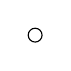
\begin{tikzpicture}[scale=0.25]
  \filldraw[fill=mTan] (1,1) circle (1em);
  \end{tikzpicture}
}
\newcommand{\bp}{\blackPebble}
\renewcommand{\wp}{\whitePebble}

\title{Decision Problems in Invertible Automata}
\date{May 10, 2017}
\author{Evan Bergeron \& Klaus Sutner}
\institute{Carnegie Mellon University}
\begin{document}

\maketitle

\begin{frame}[standout]
  What is your research?
\end{frame}

\begin{frame}{What is your research?}
  Geometric group theory, from a computer scientist's view!
\end{frame}

\begin{frame}{What is your research?}
  Automata theory turns out to be pretty useful for some recent
  developments in abstract algebra. Putting 251 and CDM to good use!
\end{frame}

\begin{frame}[standout]
  What did you prove?
\end{frame}

% TODO space out these small caps more
\begin{frame}{What did you prove?}
  Three major results:
  \begin{itemize}
  \item \textsc{membership} testing is decidable in the commutative
    case.
  \item \textsc{IsGroup} is decidable in the commutative case.
  \item A \textsc{knapsack} variant is undecidable.
  \end{itemize}
  We'll focus on the last one for this talk.
\end{frame}

\section{Some quick background}

\begin{frame}
  An \emph{automaton} looks like this:
  \begin{center}
    \includegraphics[scale=0.4]{../figures/grigorchuk}
  \end{center}
\end{frame}

\begin{frame}
  Each state corresponds with a function mapping strings to strings.
  \begin{center}
    \includegraphics[scale=0.4]{../figures/grigorchuk}
  \end{center}
\end{frame}

\begin{frame}
  Starting at the middle state, on input ``1100'', we output ``1101.''
  \begin{center}
    \includegraphics[scale=0.4]{../figures/grigorchuk}
  \end{center}
\end{frame}

\begin{frame}
  Since states are functions, we can compose them.
  \begin{center}
    \includegraphics[scale=0.4]{../figures/grigorchuk}
  \end{center}
\end{frame}

\begin{frame}
  Composing the left corner with itself yields the identity function.
  \begin{center}
    \includegraphics[scale=0.4]{../figures/grigorchuk}
  \end{center}
\end{frame}

\begin{frame}{Some notation}
  If $s$ is the function for some state, $s^i$ is the function
  corresponding to running that state $i$ times.

  If $s$ and $s'$ are function for two states, $s s'$ is the
  composition of $s$ and $s'$, first running $s$, then $s'$.
\end{frame}

\begin{frame}{Knapsack definition}
  Given as input state functions $s_1 \ldots s_k$ and a target
  function $s$, do there exist natural numbers $a_1\ldots a_k$ such
  that
  \[ s_1^{a_1} \cdots s_k^{a_K} = s \]
\end{frame}

\begin{frame}
  This turns out to be undecidable. We'll reduce from Hilbert's tenth
  problem.
\end{frame}

\begin{frame}{Hilbert's Tenth Problem}
  Define \textsc{hilbert} as following:

  Given a polynomial
  $P(x_1, \ldots, x_n) \in \mathbb{Z}[x_1, \ldots, x_n]$ and an
  integer $a$, do there exist values $y_i \in \mathbb{N}$ such that
  $P(y_1, \ldots, y_n) = a$?

  (There exist polynomials for which this is undecidable).
\end{frame}

\begin{frame}{The reduction}
  A running example for clarity's sake:
  \begin{align*}
    P(x) &= x^2 - x + 7, \\
    a &= -5
  \end{align*}
\end{frame}

% \begin{frame}[fragile]{The reduction}
%   \begin{lstlisting}[language=Python]
%     def hilbert(P): 
%   \end{lstlisting}
% \end{frame}

\begin{frame}{First, force all coefficients to be postive.}
  $x^2 - x + 7 = -5$

  if and only if

  $x^2 + 12 = x$
\end{frame}

\begin{frame}{Second, generate a system of equations.}
  Each equation will look like
  \begin{itemize}
  \item $x + y = z$,
  \item $x = c$, or 
  \item $x\cdot y = z$.
  \end{itemize}
\end{frame}

\begin{frame}{Second, generate a system of equations.}
  For example,
  \[ x^2 + 12 = x \]

  if and only if \emph{there exist} $x_i$'s such that
  \begin{align*}
    x_1 &= x, \\
    x_2 &= x * x_1, \\
    x_3 &= x_2 + 12, \text{ and} \\
    x_3 &= x.
  \end{align*}
  
\end{frame}

\begin{frame}{Third, model each equation with automata.} 
  Addition can be represented using the adding machine:
  \begin{center}
    \includegraphics[scale=0.5]{../figures/adder}
  \end{center}
  If $a$ is the left state, $x + y = z$ if and only if
  $a^x a^y = a^z$.
\end{frame}

\begin{frame}{Third, model each equation with automata.} 
  Constant equality also uses the adding machine.
  \begin{center}
    \includegraphics[scale=0.5]{../figures/adder}
  \end{center}
  $x = c$ if and only if $a^x= a^c$.
\end{frame}

\begin{frame}{Third, model each equation with automata.} 
  Multiplication can be represented using the Heisenberg semigroup:
  \begin{align*}
    H_3(\mathbb{N}) = \left\{
    \begin{bmatrix}
      1 & a & c \\
      0 & 1 & b \\
      0 & 0 & 1
    \end{bmatrix};
    a, b, c \in \mathbb{N}
    \right\}
  \end{align*}
  (Multiplication of matrices of this form can be represented with
  automata).
\end{frame}

\begin{frame}{The multiplication trick}
  \[
    H^x_{1,0,0} H^y_{0,0,1} =
    \begin{bmatrix}
      1 & x & xy \\
      0 & 1 & y \\
      0 & 0 & 1
    \end{bmatrix} = 
    \begin{bmatrix}
      1 & x & z \\
      0 & 1 & y \\
      0 & 0 & 1
    \end{bmatrix} = 
    H^z_{1,0,0} H^y_{0,0,1} H^x_{1,0,0}
  \]
where
\[
  H_{x,y,z} = 
      \begin{bmatrix}
        1 & x & z \\
        0 & 1 & y \\
        0 & 0 & 1
      \end{bmatrix}
\]
Then $x\cdot y = z$ iff
$H^x_{1,0,0} H^y_{0,0,1} = H^z_{1,0,0} H^y_{0,0,1} H^x_{1,0,0}$.
\end{frame}

% \begin{frame}{Our running example}
%   \[ x^2 + 12 = x \]
%   if and only if \emph{there exist} $x_i$'s such that
%   % Our equations have transformed:
%   \begin{align*}
%     x_1 &= x \longrightarrow  &a^{x_1} = a^x\\
%     x_2 &= x * x_1 \longrightarrow &H^x_{1,0,0} H^{x_2}_{0,0,1} = H^{x_1}_{1,0,0} H^{x_2}_{0,0,1} H^x_{1,0,0} \\
%     x_3 &= x_2 + 12 \longrightarrow &a^{x_3} = a^{x_2}a^{12}\\
%     x_3 &= x \longrightarrow &a^{x_3}a^{x}
%   \end{align*}
% \end{frame}

\begin{frame}{Our running example previously}
  \[ x^2 + 12 = x \]
  if and only if \emph{there exist} $x_i$'s such that
  \begin{align*}
    x_1 &= x\\
    x_2 &= x * x_1\\
    x_3 &= x_2 + 12\\
    x_3 &= x
  \end{align*}
\end{frame}

\begin{frame}{Our running example now}
  \[ x^2 + 12 = x \]
  if and only if \emph{there exist} $x_i$'s such that
  \begin{align*}
    a^{x_1} &= a^x& \text{in $\mathbb{N}$}\\
    H^x_{1,0,0} H^{x_2}_{0,0,1} &= H^{x_1}_{1,0,0} H^{x_2}_{0,0,1} H^x_{1,0,0} & \text{in $H_3(\mathbb{N})$}\\
    a^{x_3} &= a^{x_2}a^{12}& \text{in $\mathbb{N}$}\\
    a^{x_3} &= a^{x}& \text{in $\mathbb{N}$}
  \end{align*}
\end{frame}

\begin{frame}{Lastly, combine into a single equation.}
  \[ x^2 + 12 = x \]
  if and only if \emph{there exist} $x_i$'s such that
  \begin{align*}
    (a^{x_1}, H^x_{1,0,0} H^{x_2}_{0,0,1}, a^{x_3}, a^{x_3}) = 
    (a^x, H^{x_1}_{1,0,0} H^{x_2}_{0,0,1} H^x_{1,0,0}, a^{x_2}a^{12}, a^{x})
  \end{align*}
  in $(\mathbb{N}, H_3(\mathbb{N}), \mathbb{N}, \mathbb{N})$.

  (This corresponds with taking the product machine of different
  machines).
\end{frame}

\begin{frame}{Recap}
  On input polynomial $P$,
  \begin{enumerate}
  \item Separate into positive and negative parts.
  \item Generate system of equations.
  \item Model each equation with an automaton.
  \item Take product of all equations, feed to \textsc{knapsack}
    oracle.
  \end{enumerate}
\end{frame}

\begin{frame}[standout]
  Questions?
\end{frame}

\begin{frame}[standout]
  Thanks!
\end{frame}

\end{document}